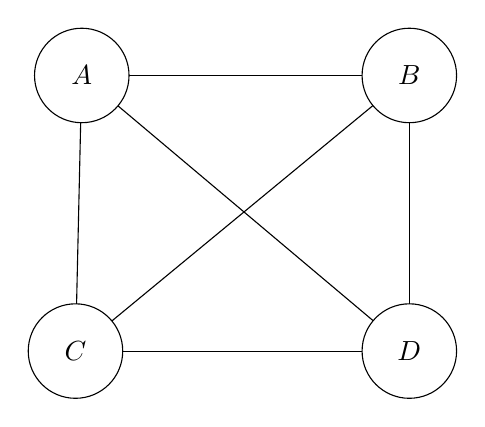
\begin{tikzpicture}[scale=0.2]
	\tikzstyle{every node}+=[inner sep=0pt]
	\draw [black] (21.8,-10.8) circle (3);
	\draw (21.8,-10.8) node {$A$};
	\draw [black] (42.6,-10.8) circle (3);
	\draw (42.6,-10.8) node {$B$};
	\draw [black] (42.6,-28.3) circle (3);
	\draw (42.6,-28.3) node {$D$};
	\draw [black] (21.4,-28.3) circle (3);
	\draw (21.4,-28.3) node {$C$};
	\draw [black] (39.6,-10.8) -- (24.8,-10.8);
	\draw [black] (21.73,-13.8) -- (21.47,-25.3);
	\draw [black] (24.4,-28.3) -- (39.6,-28.3);
	\draw [black] (42.6,-25.3) -- (42.6,-13.8);
	\draw [black] (40.29,-12.71) -- (23.71,-26.39);
	\draw [black] (24.1,-12.73) -- (40.3,-26.37);
\end{tikzpicture}